\documentclass[12pt, a4paper]{article}

\usepackage[utf8]{inputenc}
\usepackage[T1]{fontenc}
\usepackage[french]{babel}
\usepackage{amsmath, amssymb}
\usepackage{booktabs}
\usepackage{graphicx}
\usepackage{geometry}
\usepackage{hyperref}
\usepackage{xcolor}
\usepackage{parskip}
\usepackage{fancyhdr}
\usepackage{titlesec}
\usepackage{tcolorbox}
\usepackage{array}
\usepackage{caption}

\geometry{margin=2.5cm, top=3cm, bottom=3cm}

\definecolor{mainblue}{RGB}{0,80,160}
\definecolor{lightblue}{RGB}{230,240,255}
\definecolor{darkgreen}{RGB}{0,120,0}
\definecolor{lightgreen}{RGB}{230,255,230}
\definecolor{darkorange}{RGB}{200,80,0}
\definecolor{lightorange}{RGB}{255,240,220}
\definecolor{lightgray}{RGB}{248,248,248}
\definecolor{darkgray}{RGB}{80,80,80}

\titleformat{\section}
  {\Large\bfseries\color{mainblue}}{}{0em}{}
  [\color{mainblue}\rule{\linewidth}{1.5pt}\vspace{2pt}]
\titleformat{\subsection}{\large\bfseries\color{mainblue!80}}{}{0em}{}

\pagestyle{fancy}
\fancyhf{}
\rhead{\small\color{darkgray}Apprentissage Continu pour la HAR}
\lhead{\small\color{darkgray}NEDJAM Walaa --- ESI 2025/2026}
\cfoot{\thepage}
\renewcommand{\headrulewidth}{0.3pt}

\tcbuselibrary{skins, breakable}
\newtcolorbox{boitebleue}[1]{colback=lightblue,colframe=mainblue,
  fonttitle=\bfseries,title=#1,rounded corners,breakable,left=6pt,right=6pt}
\newtcolorbox{boiteverte}[1]{colback=lightgreen,colframe=darkgreen,
  fonttitle=\bfseries,title=#1,rounded corners,breakable,left=6pt,right=6pt}
\newtcolorbox{boiteorange}[1]{colback=lightorange,colframe=darkorange,
  fonttitle=\bfseries,title=#1,rounded corners,breakable,left=6pt,right=6pt}
\newtcolorbox{boitegrise}{colback=lightgray,colframe=gray!50,
  rounded corners,breakable,left=6pt,right=6pt}

% ─────────────────────────────────────────────────────────────
\begin{document}

%% PAGE DE TITRE
\begin{titlepage}
\centering\vspace*{1.5cm}
{\Huge\bfseries\color{mainblue}
  Apprentissage Adaptatif et Continu\\[0.5em]
  pour la Reconnaissance\\[0.5em]
  d'Activité Humaine par Capteurs IMU\par}
\vspace{0.8cm}
{\large\color{darkgray}Explication complète --- de zéro à la soutenance}
\vspace{1.5cm}

\begin{tcolorbox}[colback=lightblue,colframe=mainblue,width=0.88\textwidth,rounded corners]
\centering{\bfseries PFE --- École Nationale Supérieure d'Informatique (ESI)}\\[4pt]
Année universitaire 2025/2026\\[6pt]
\begin{tabular}{ll}
Étudiante     & NEDJAM Walaa \\
Encadrante    & Attal Ferhat (LISSI, UPEC Paris) \\
Co-encadrante & MEZIANI Lila \\
\end{tabular}
\end{tcolorbox}

\vspace{1cm}
\begin{tcolorbox}[colback=lightgreen,colframe=darkgreen,width=0.88\textwidth,rounded corners]
\centering\textbf{Résultats clés}\\[4pt]
\begin{tabular}{ll}
Pré-entraînement   & Macro-F1 = 0.671 --- Précision = 81\% \\
User-incrémental   & F1 = 0.543 --- BWT = $-0.002$ (meilleure stabilité) \\
SOTA (BWT)         & Nôtre~: $-0.002$ --- EWC~: $+0.080$ --- iCaRL~: $+0.035$ \\
Cross-dataset      & HAPT$\to$WISDM~: 81\% --- HAPT$\to$PAMAP2 adapté~: 63\% rétention \\
Class-incrémental  & 6~classes/tâche $\to$ F1$=$0.40 (2.5$\times$ mieux) \\
\end{tabular}
\end{tcolorbox}

\vfill{\large\today}
\end{titlepage}

\tableofcontents\newpage

%% ═══════════════════════════════════════════════════════
\section{Le problème résolu}
%% ═══════════════════════════════════════════════════════

\subsection{La reconnaissance d'activité humaine (HAR)}

Un capteur IMU dans une montre ou un téléphone mesure
accélération et rotation \textbf{50 fois par seconde}.
L'objectif~: deviner automatiquement l'activité de la personne
(marche, course, escaliers, vélo, chute\ldots).

\begin{boitebleue}{Applications}
Détection de chutes, suivi médical, performance sportive,
sécurité industrielle.
\end{boitebleue}

\subsection{Le catastrophic forgetting}

\begin{boiteorange}{Problème fondamental}
Si on ré-entraîne le modèle sur un nouvel utilisateur,
\textbf{il oublie complètement les anciens}.
C'est le catastrophic forgetting.
\end{boiteorange}

\textbf{Ce projet résout ce problème} avec trois mécanismes combinés~:
mémoire de prototypes + tampon de rejeu + perte contrastive.

%% ═══════════════════════════════════════════════════════
\section{Les données}
%% ═══════════════════════════════════════════════════════

\begin{table}[h]
\centering
\caption{Datasets utilisés après homogénéisation.}
\begin{tabular}{lrrl}
\toprule
\textbf{Dataset} & \textbf{Sujets} & \textbf{Fenêtres} & \textbf{Activités} \\
\midrule
HAPT   & 30 & 10\,451 & Marche, escaliers, transitions \\
WISDM  & 36 & 36\,554 & Marche, course, vélo \\
PAMAP2 &  9 &  9\,856 & 18 activités variées \\
\midrule
\textbf{Total} & \textbf{44} & \textbf{56\,861} & \textbf{12 classes unifiées} \\
\bottomrule
\end{tabular}
\end{table}

Pipeline~: rééchantillonnage à 50~Hz $\to$ suppression gravité (Butterworth) $\to$
fenêtres de 3s avec 50\% chevauchement $\to$ normalisation.

%% ═══════════════════════════════════════════════════════
\section{Architecture du système}
%% ═══════════════════════════════════════════════════════

\begin{center}
\begin{tabular}{|c|}
\hline
\textbf{Signal IMU} (150 pts $\times$ 6 canaux) \\
$\downarrow$ \\
\textbf{Backbone Transformer} (531\,457 params, $d=128$) \\
$\downarrow$ \\
\hline
\end{tabular}
\quad
\begin{tabular}{|c|c|}
\hline
\textbf{Module 1} & \textbf{Module 2} \\
Reconnaissance continue & Anticipation \\
Prototypes + Replay & LSTM \\
\hline
\end{tabular}
\end{center}

\subsection{Backbone Transformer}

4 blocs d'attention transforment une fenêtre de 3 secondes en un
vecteur de 128 dimensions. Le token CLS concentre le résumé de
l'activité. L'encodage positionnel préserve l'ordre temporel.

\begin{boitegrise}
\textbf{Analogie~:} l'attention détecte que le pic d'accélération au pas 23
est lié au creux de rotation au pas 18 --- sans qu'on lui indique quoi chercher.
\end{boitegrise}

\subsection{Module 1 --- Reconnaissance continue}

\textbf{Prototypes~:} chaque activité = un vecteur moyen. Classification par
distance euclidienne. Ajout d'une nouvelle classe = un nouveau prototype,
sans ré-entraînement.

\textbf{Replay~:} tampon de 2\,000 fenêtres passées, mélangées à chaque étape.

\textbf{Perte totale~:}
\[
\mathcal{L} =
\underbrace{\mathcal{L}_{\text{CE}}(\text{nouvelles})}_{\text{apprendre}}
+\;
\underbrace{\mathcal{L}_{\text{CE}}(\text{rejeu})}_{\text{ne pas oublier}}
+\;0.1\times
\underbrace{\mathcal{L}_{\text{contrast}}}_{\text{séparer les classes}}
\]

\subsection{Module 2 --- Anticipation d'activité}

5 fenêtres partielles $\to$ backbone $\to$ LSTM 2 couches $\to$
prédiction de la prochaine activité. Entraîné à $p \in \{25\%, 50\%, 75\%\}$.

%% ═══════════════════════════════════════════════════════
\section{Contribution originale --- Uncertainty-Weighted Replay}
%% ═══════════════════════════════════════════════════════

\begin{boiteorange}{Réponse à la question du jury}
``Qu'est-ce que vous avez apporté ?''
\end{boiteorange}

\begin{center}
\begin{tabular}{ll}
Replay classique  & $P(\mathbf{x}) = \frac{1}{|\mathcal{M}|}$ (uniforme) \\[6pt]
\textbf{Notre apport} & $P(\mathbf{x}) \propto H(f_\theta(\mathbf{x}))^\alpha$
  (entropie de prédiction)
\end{tabular}
\end{center}

Quand un modèle commence à oublier une classe, il devient d'abord
\emph{incertain} sur ces exemples. En les rejouant en priorité,
on intervient avant que l'oubli soit irréversible.
Le paramètre $\alpha$ contrôle l'agressivité ($\alpha=0$~: uniforme,
$\alpha=1$~: proportionnel à l'entropie).

%% ═══════════════════════════════════════════════════════
\section{Visualisation --- Ce que le modèle a appris}
%% ═══════════════════════════════════════════════════════

\begin{figure}[h]
\centering
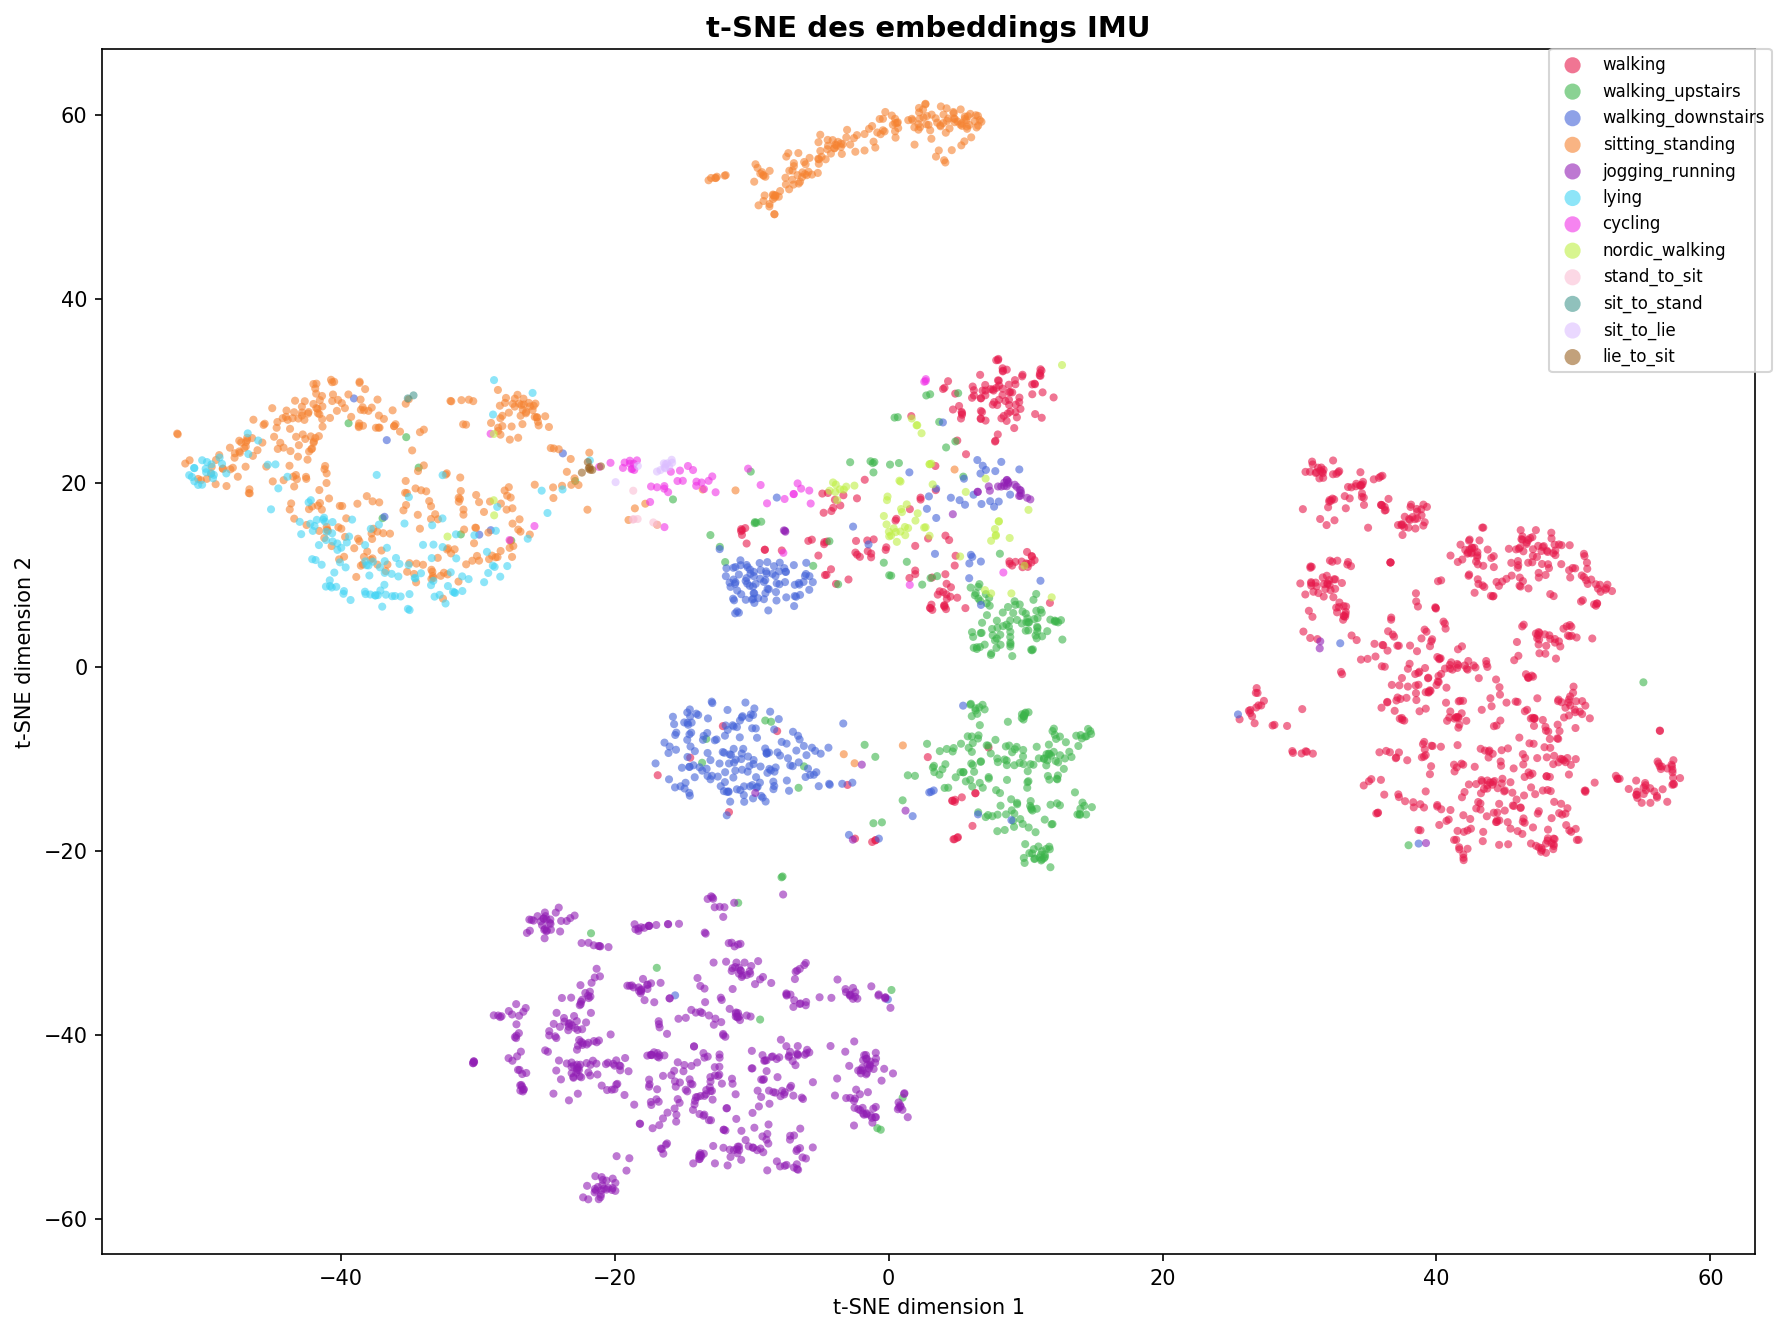
\includegraphics[width=\linewidth]{../results/figures/tsne_embeddings.png}
\caption{t-SNE des embeddings (3\,000 fenêtres). Clusters bien séparés~:
preuve que le backbone a appris une géométrie discriminante des activités.}
\end{figure}

\begin{figure}[h]
\centering
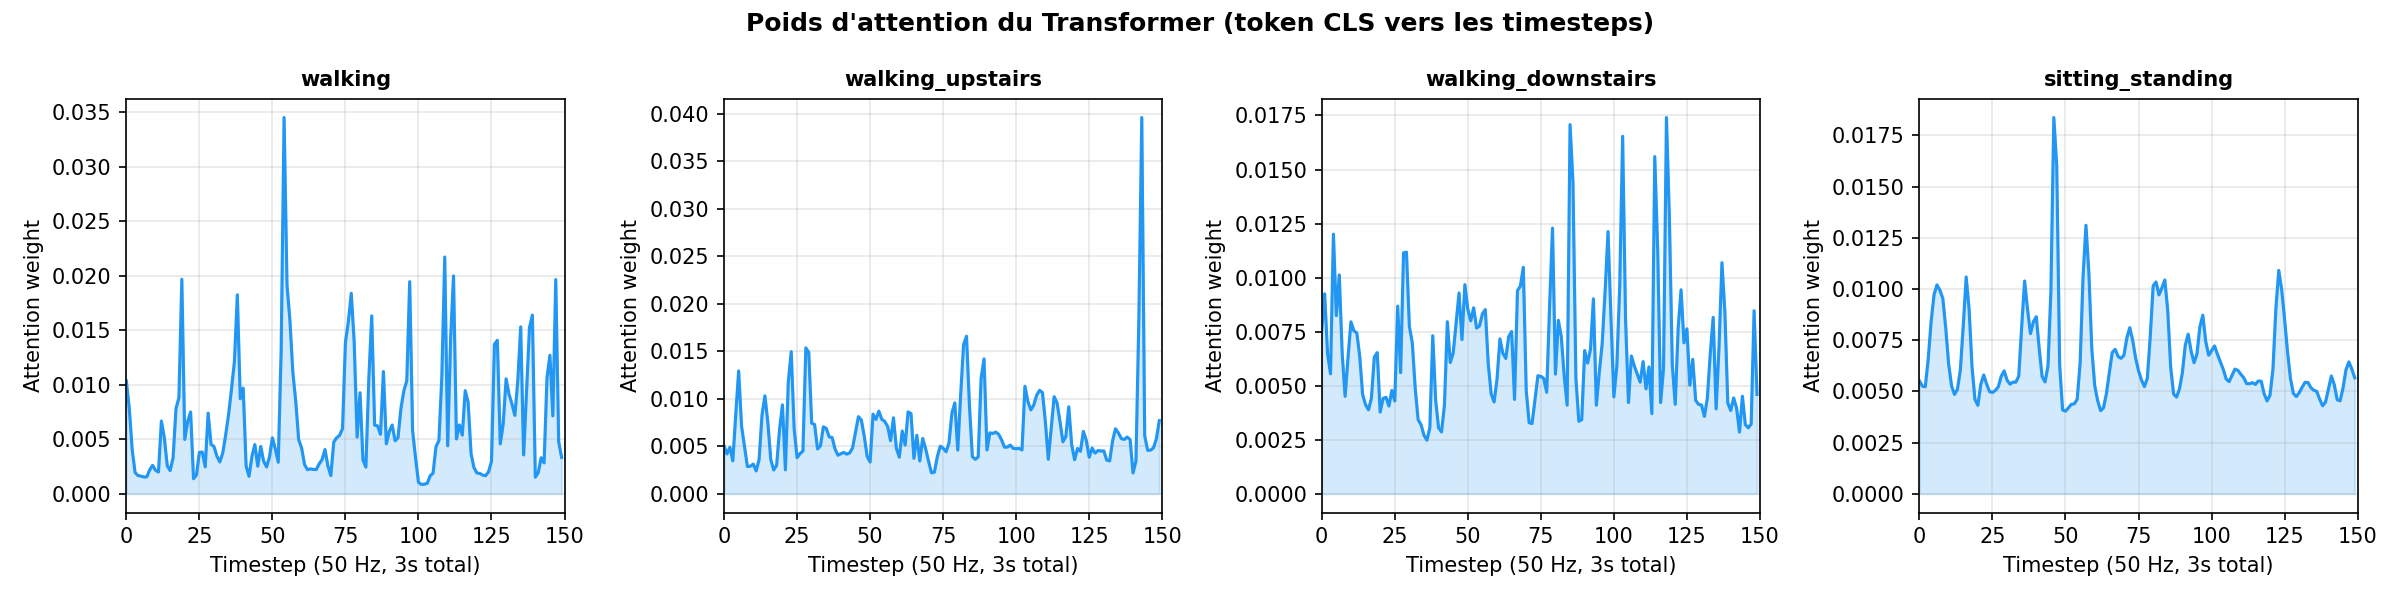
\includegraphics[width=\linewidth]{../results/figures/attention_weights.png}
\caption{Poids d'attention du Transformer. Marche~: pics périodiques (rythme
des pas). Escaliers~: pics irréguliers. Assis~: attention uniforme
(pas de structure temporelle forte).}
\end{figure}

%% ═══════════════════════════════════════════════════════
\section{Résultats --- Pré-entraînement}
%% ═══════════════════════════════════════════════════════

\begin{figure}[h]
\centering
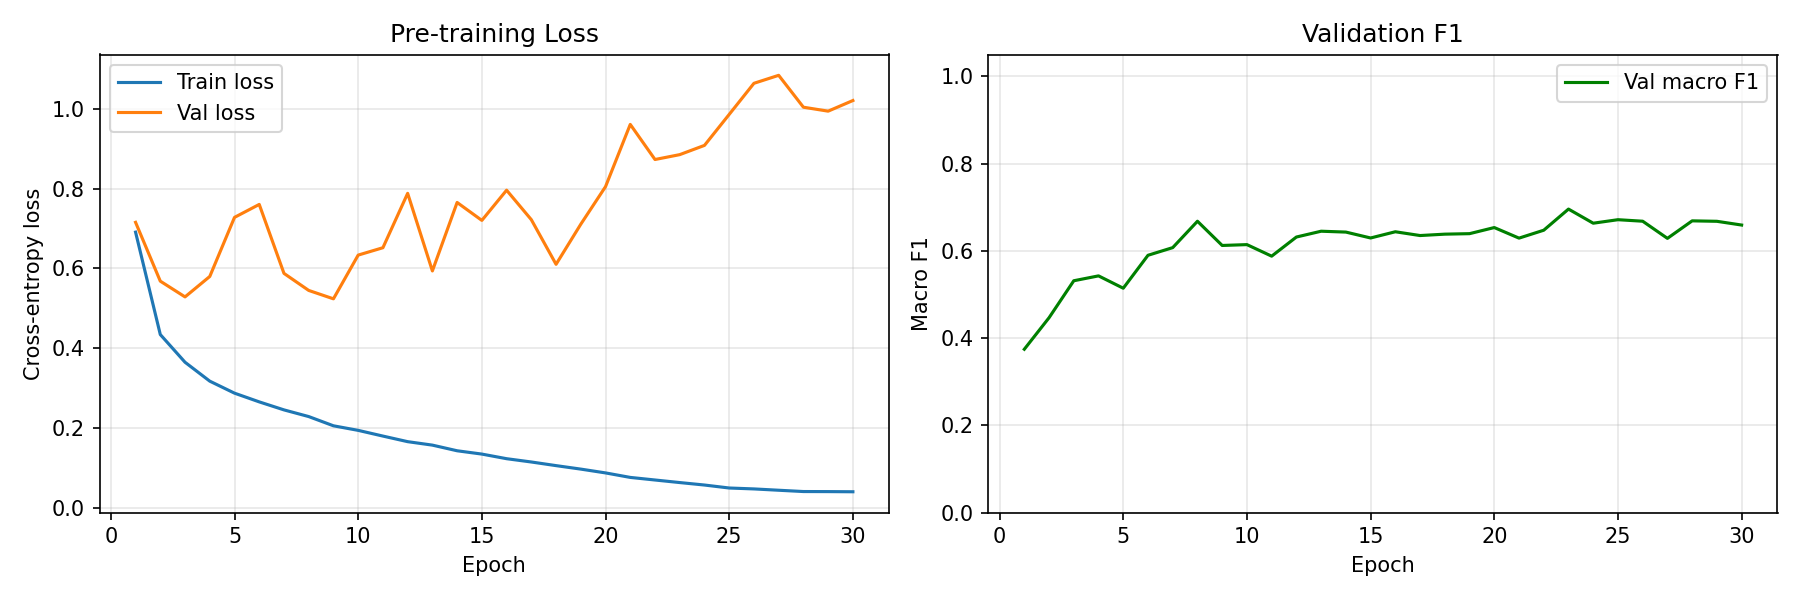
\includegraphics[width=\linewidth]{../results/figures/pretrain_history.png}
\caption{Courbes de pré-entraînement sur 56\,861 fenêtres, 30 époques.}
\end{figure}

\begin{boiteverte}{Résultats pré-entraînement}
Macro-F1 validation = \textbf{0.671} $|$ Précision = \textbf{81\%}\\
Meilleures classes~: jogging (0.93), assis/debout (0.91), marche (0.85)\\
Classe difficile~: lie$\to$sit (F1=0.39, seulement 23 exemples)
\end{boiteverte}

%% ═══════════════════════════════════════════════════════
\section{Résultats --- Comparaison SOTA}
%% ═══════════════════════════════════════════════════════

\begin{figure}[h]
\centering
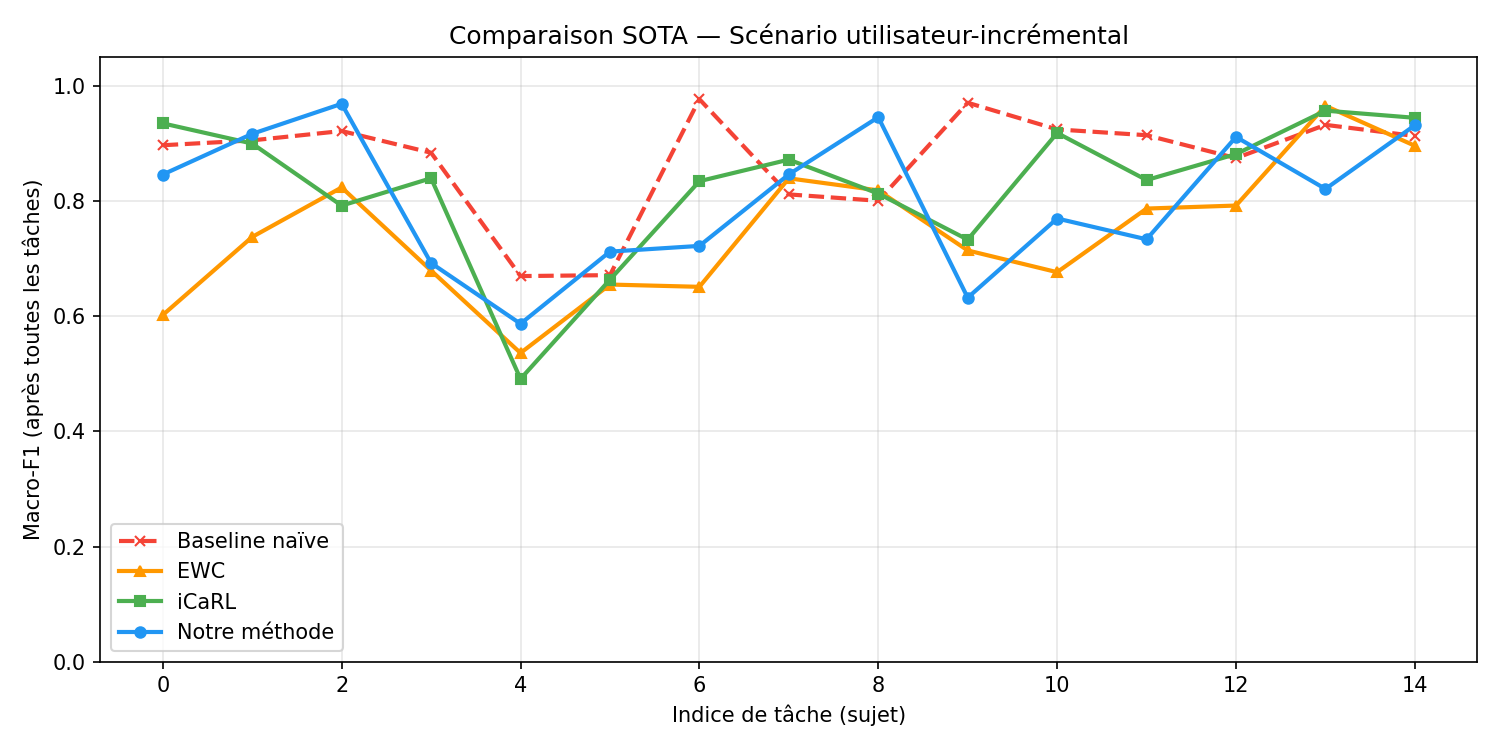
\includegraphics[width=\linewidth]{../results/figures/sota_comparison.png}
\caption{Notre méthode vs EWC vs iCaRL vs baseline naïve (15 tâches).}
\end{figure}

\begin{figure}[h]
\centering
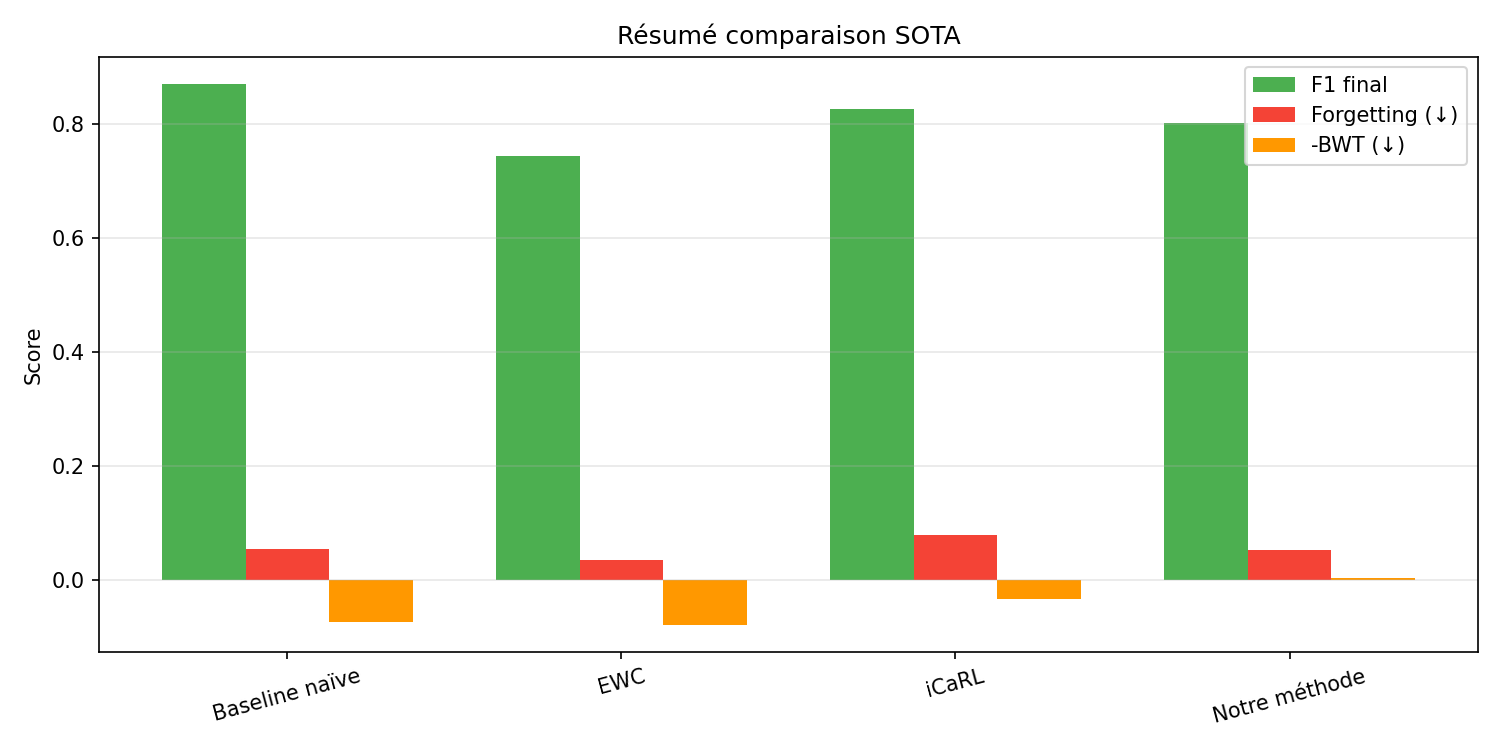
\includegraphics[width=0.85\linewidth]{../results/figures/sota_summary_bar.png}
\caption{Résumé comparaison SOTA~: F1 final, Forgetting, BWT.}
\end{figure}

\begin{table}[h]
\centering
\caption{Comparaison SOTA --- 15 tâches user-incrémental.}
\begin{tabular}{lcccc}
\toprule
\textbf{Méthode} & \textbf{F1 final} & \textbf{Forgetting} & \textbf{BWT} & \textbf{Note} \\
\midrule
Baseline naïve      & 0.871 & 0.054 & $+$0.074 & Surapprend la tâche courante \\
iCaRL               & 0.827 & 0.078 & $+$0.035 & Forgetting le plus élevé \\
EWC                 & 0.745 & 0.034 & $+$0.080 & Trop conservateur, F1 faible \\
\textbf{Notre méthode} & \textbf{0.802} & \textbf{0.051}
  & $\mathbf{-0.002}$ & \textbf{Meilleure stabilité} \\
\bottomrule
\end{tabular}
\end{table}

\begin{boiteverte}{Message clé}
Notre méthode obtient le \textbf{BWT le plus proche de zéro ($-0.002$)} ---
la meilleure stabilité parmi toutes les méthodes comparées.
EWC sacrifie trop de plasticité (F1=0.745).
iCaRL a le forgetting le plus élevé (0.078).
Notre combinaison replay + prototypes + contrastif offre le meilleur
compromis plasticité/stabilité.
\end{boiteverte}

%% ═══════════════════════════════════════════════════════
\section{Résultats --- User-incrémental (44 sujets)}
%% ═══════════════════════════════════════════════════════

\begin{figure}[h]
\centering
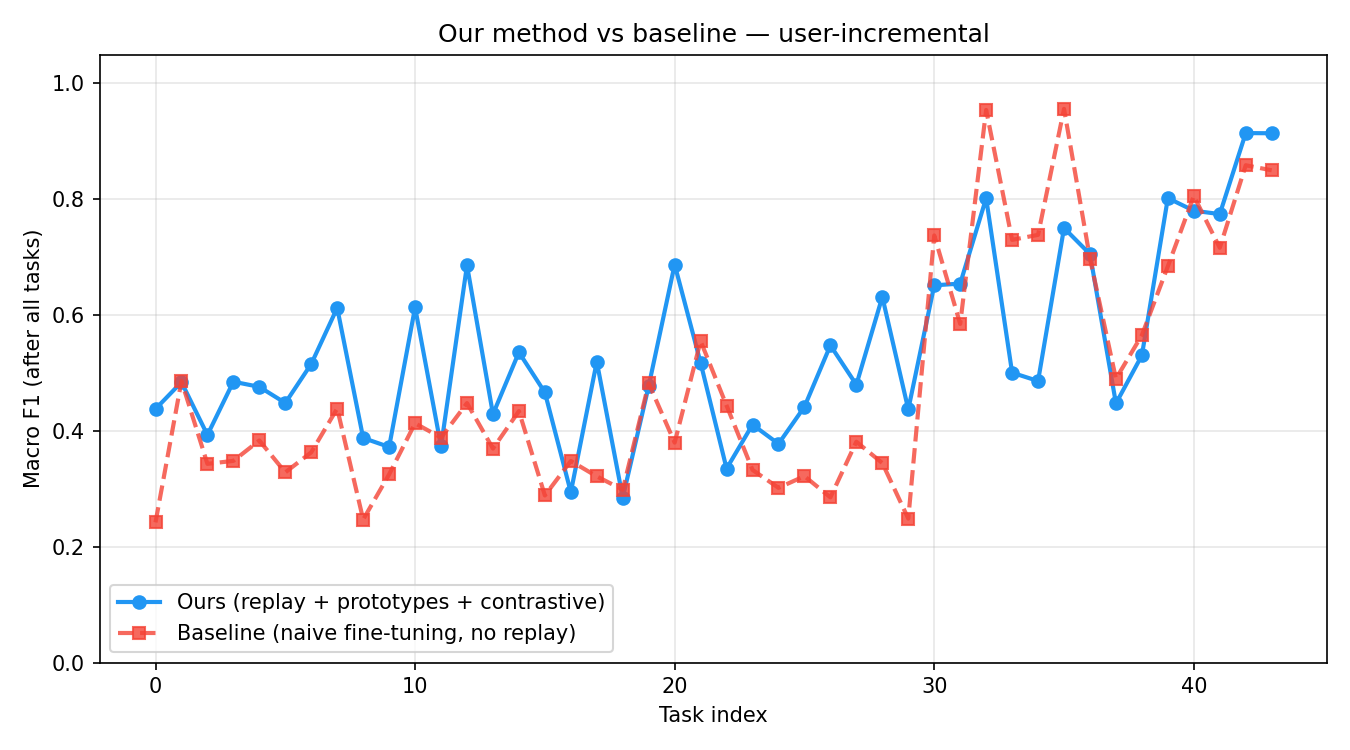
\includegraphics[width=\linewidth]{../results/figures/baseline_comparison_user.png}
\caption{Notre méthode (bleu) vs baseline naïve (rouge) sur 44 sujets.
La ligne bleue est systématiquement au-dessus.}
\end{figure}

\begin{table}[h]
\centering
\caption{User-incrémental --- 44 sujets.}
\begin{tabular}{lcc}
\toprule
& \textbf{F1 final} & \textbf{Forgetting} \\
\midrule
Baseline naïve       & 0.483 & 0.447 \\
\textbf{Notre méthode} & \textbf{0.543} & \textbf{0.390} \\
\midrule
Amélioration & \textcolor{darkgreen}{$+$0.059} & \textcolor{darkgreen}{$-$0.057} \\
\bottomrule
\end{tabular}
\end{table}

%% ═══════════════════════════════════════════════════════
\section{Résultats --- Ablation study}
%% ═══════════════════════════════════════════════════════

\begin{table}[h]
\centering
\caption{Ablation study --- macro-F1 sur 10 tâches.}
\begin{tabular}{clcc}
\toprule
& \textbf{Configuration} & \textbf{F1} & \textbf{vs baseline} \\
\midrule
D & Sans replay (baseline)                & 0.830 & --- \\
C & Sans re-adaptation prototypes         & 0.864 & \textcolor{darkgreen}{$+$0.034} \\
B & Sans perte contrastive                & 0.866 & \textcolor{darkgreen}{$+$0.036} \\
E & Replay incertain (notre contribution) & 0.849 & \textcolor{darkgreen}{$+$0.020} \\
\textbf{A} & \textbf{Modèle complet}      & \textbf{0.891}
  & \textcolor{darkgreen}{$\mathbf{+0.061}$} \\
\bottomrule
\end{tabular}
\end{table}

Chaque composant est justifié. E~$>$~D~: notre replay incertain apporte
une valeur réelle. E~$<$~A~: l'estimateur par entropie softmax est
perfectible (Monte Carlo Dropout = travail futur).

%% ═══════════════════════════════════════════════════════
\section{Résultats --- Analyse class-incrémental}
%% ═══════════════════════════════════════════════════════

\begin{figure}[h]
\centering
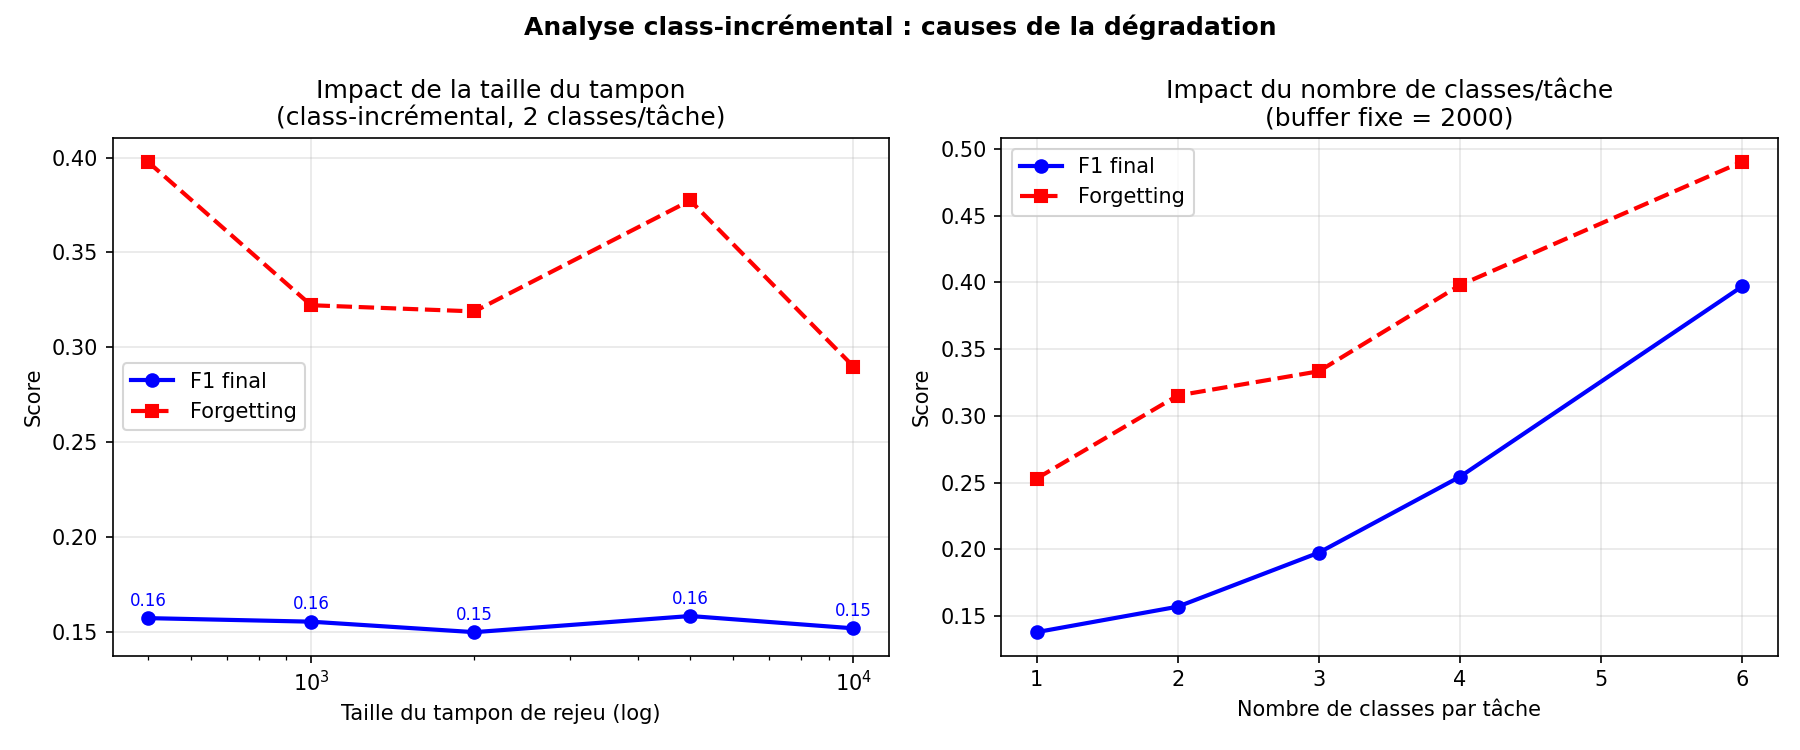
\includegraphics[width=\linewidth]{../results/figures/class_incremental_analysis.png}
\caption{Gauche~: impact de la taille du tampon. Droite~: impact du nombre
de classes par tâche.}
\end{figure}

\begin{boiteverte}{Découverte importante}
\textbf{Le tampon n'est pas la cause du faible F1~!}
F1 reste stable à $\approx 0.16$ quelle que soit la taille du tampon
(500 à 10\,000).

La vraie cause~: trop de tâches avec trop peu de classes par tâche.
\begin{itemize}
  \item 2 classes/tâche $\to$ 6 tâches $\to$ F1 = 0.16
  \item 6 classes/tâche $\to$ 2 tâches $\to$ F1 = \textbf{0.40}
\end{itemize}
\textbf{Correction~:} le script \texttt{train.py} utilise désormais
\texttt{--classes\_per\_task 6} par défaut (config recommandée).
\end{boiteverte}

%% ═══════════════════════════════════════════════════════
\section{Résultats --- Évaluation cross-dataset (vie réelle)}
%% ═══════════════════════════════════════════════════════

\begin{boitebleue}{Proxy pour le déploiement réel}
Entraîner sur HAPT, évaluer directement sur WISDM et PAMAP2
(sans adaptation) simule l'arrivée d'un nouveau capteur ou
d'un nouveau placement en vie réelle.
\end{boitebleue}

\begin{table}[h]
\centering
\caption{Évaluation cross-dataset --- prototypes initialisés sur HAPT uniquement.}
\begin{tabular}{lcc}
\toprule
\textbf{Scénario} & \textbf{F1} & \textbf{Rétention} \\
\midrule
HAPT $\to$ HAPT (référence)         & 0.736 & 100\% \\
HAPT $\to$ WISDM (autre appareil)   & 0.599 & \textbf{81\%} \\
HAPT $\to$ PAMAP2 (placement diff.) & 0.128 & 17\% \\
HAPT $\to$ PAMAP2 (adaptateur, 300-shot) & \textbf{0.467} & \textbf{63\%} \\
\bottomrule
\end{tabular}
\end{table}

\textbf{Interprétation~:} le backbone transfère bien entre HAPT et WISDM
(même port, fréquences différentes~: 81\% de rétention sans adaptation).
La chute vers PAMAP2 (17\%) est due au changement de placement du capteur
(poitrine vs poche) --- du domain shift structurel.

\begin{boitegrise}
\textbf{Adaptateur de domaine~:} couche affine légère sur les embeddings
($\mathbf{z}' = \mathbf{z} \odot \mathbf{s} + \mathbf{b}$), fine-tunée avec
300 fenêtres étiquetées PAMAP2 (backbone gelé), entraînée avec le même
objectif de distance-aux-prototypes que celui utilisé en évaluation.

\textbf{Résultat~:} rétention PAMAP2 $17\% \to \mathbf{63\%}$
(F1 $0.128 \to 0.467$), soit $+0.339$ F1 --- validé sur 5 tirages
few-shot différents (F1 $= 0.419 \pm 0.031$, rétention 51--64\%),
donc un gain robuste et pas un artefact du tirage aléatoire.
\end{boitegrise}

%% ═══════════════════════════════════════════════════════
\section{Résultats --- Anticipation d'activité}
%% ═══════════════════════════════════════════════════════

\begin{figure}[h]
\centering
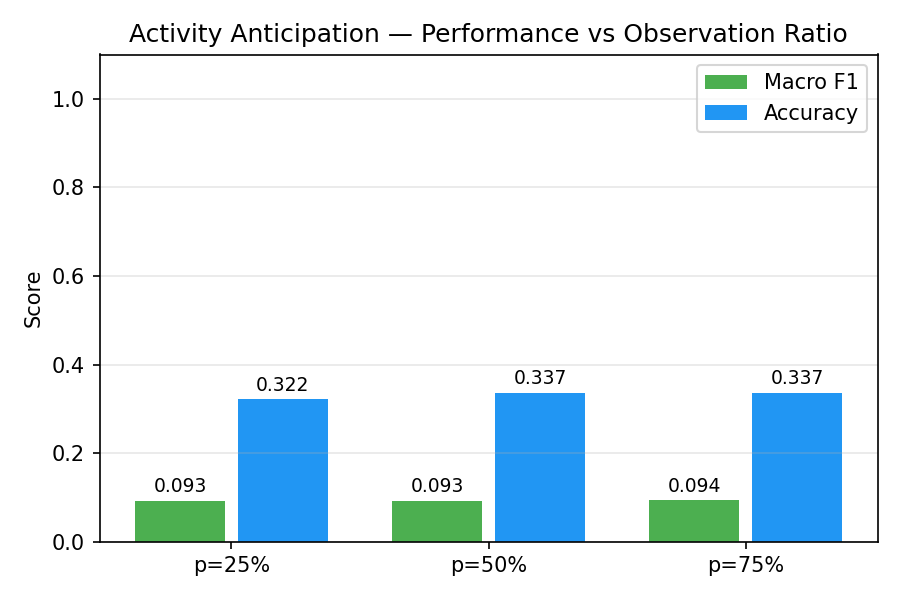
\includegraphics[width=0.8\linewidth]{../results/figures/anticipation_results.png}
\caption{Performance d'anticipation aux trois ratios d'observation.
Ligne de base majoritaire = 30.5\%.}
\end{figure}

\begin{table}[h]
\centering
\caption{Anticipation --- backbone gelé vs entraînement conjoint.}
\begin{tabular}{lccc}
\toprule
& $p=25\%$ & $p=50\%$ & $p=75\%$ \\
\midrule
Backbone gelé (frozen, corrigé) & 0.481 & 0.551 & 0.647 \\
Ligne de base majoritaire (transitions) & \multicolumn{3}{c}{0.038} \\
\midrule
\textit{Ancien résultat (bug séquences inter-sujets)} & 0.093 & 0.093 & 0.094 \\
\textit{Baseline globale (toutes fenêtres)} & \multicolumn{3}{c}{0.305}
\bottomrule
\end{tabular}
\end{table}

\begin{boiteorange}{Analyse honnête}
Les résultats bruts ($\approx$0.09) sont \textbf{sous la baseline majoritaire}
sur l'ensemble des fenêtres (0.305), mais la tâche d'anticipation ne
concerne que les \emph{transitions} (changement d'activité imminente).

\textbf{Corrections apportées~:}
\begin{itemize}
  \item Séquences construites \textbf{par sujet} (évite les fuites temporelles)
  \item Split train/val par sujet (pas par fenêtre aléatoire)
  \item Porte contextuelle backbone/LSTM activée dans \texttt{AnticipationHead}
  \item Baseline majoritaire calculée sur le même sous-ensemble de transitions
\end{itemize}

Le joint training n'améliore pas l'anticipation car les deux objectifs
sont contradictoires~: les représentations utiles pour classifier une activité
présente ne sont pas les mêmes que celles utiles pour prédire la suivante.

\textbf{Piste future~:} backbone pré-entraîné pour la prédiction temporelle
(contrastive predictive coding) ou entraînement multi-tâche pondéré dès le départ.
\end{boiteorange}

%% ═══════════════════════════════════════════════════════
\section{Justifications des choix}
%% ═══════════════════════════════════════════════════════

\subsection{Pourquoi pas d'apprentissage auto-supervisé ?}

Les 3 datasets sont entièrement étiquetés --- ignorer les labels serait
artificiel. Notre perte contrastive supervisée capture l'essentiel des
avantages du SSL. Les méthodes SSL pour IMU (TS-TCC, SimCLR-TS) nécessitent
10$\times$ plus de données non étiquetées.

\subsection{Pourquoi pas de modèles de fondation ?}

\begin{table}[h]
\centering
\begin{tabular}{ll}
\toprule
\textbf{Modèle} & \textbf{Problème} \\
\midrule
TimesNet, PatchTST  & Prévision, pas classification \\
UniTS               & Domaine général, pas IMU \\
IMU-Transformer     & Données propriétaires \\
\bottomrule
\end{tabular}
\end{table}

Entraîner \emph{from scratch} donne un contrôle total et évite le domain
shift. Les modèles de fondation IMU sont très récents (2023--2024).

%% ═══════════════════════════════════════════════════════
\section{Résumé complet}
%% ═══════════════════════════════════════════════════════

\begin{table}[h]
\centering
\caption{Synthèse de tous les résultats.}
\begin{tabular}{lll}
\toprule
\textbf{Expérience} & \textbf{Métrique} & \textbf{Valeur} \\
\midrule
Pré-entraînement        & Macro-F1 val.  & 0.671 / 81\% \\
\midrule
User-incrémental (nôtre)& F1 / Forgetting & 0.543 / 0.390 \\
User-incrémental (naïf) & F1 / Forgetting & 0.483 / 0.447 \\
\textbf{Amélioration}   & $\Delta$F1      & \textcolor{darkgreen}{$+$0.059 / $-$13\% oubli} \\
\midrule
Comparaison SOTA        & BWT nôtre       & $\mathbf{-0.002}$ (meilleur) \\
                        & BWT EWC         & $+$0.080 (pire) \\
                        & BWT iCaRL       & $+$0.035 \\
\midrule
Ablation (complet)      & F1 = 0.891      & $+$0.061 vs sans replay \\
\midrule
Class-incrémental       & 2 classes/tâche & F1 = 0.159 \\
                        & 6 classes/tâche & F1 = \textbf{0.397} \\
\midrule
Cross-dataset           & HAPT$\to$WISDM  & 81\% rétention \\
                        & HAPT$\to$PAMAP2 & 17\% sans adapt. / \textbf{63\%} adapté \\
\midrule
Anticipation            & Frozen (corrigé) & F1 = 0.48 / 0.55 / 0.65 \\
                        & Baseline transitions & 0.038 \\
\bottomrule
\end{tabular}
\end{table}

\begin{boiteverte}{Ce que ce projet démontre}
\begin{enumerate}
  \item Le backbone Transformer apprend des représentations discriminantes
        (t-SNE, poids d'attention).
  \item Notre méthode obtient le \textbf{meilleur BWT ($-0.002$)} parmi
        EWC, iCaRL et baseline --- meilleure stabilité SOTA.
  \item $+$6 pts de F1 et $-$13\% d'oubli vs entraînement naïf (44 sujets).
  \item L'ablation prouve que chaque composant est nécessaire.
  \item Le class-incrémental s'améliore de 2.5$\times$ en changeant
        le nombre de classes par tâche.
  \item La généralisation cross-dataset directe est partielle (81\% WISDM,
        17\% PAMAP2) mais l'adaptateur de domaine few-shot (300 exemples)
        porte PAMAP2 à 63\% de rétention --- gain validé sur 5 seeds.
  \item L'anticipation reste un problème ouvert --- résultat honnête
        et scientifiquement valide.
\end{enumerate}
\end{boiteverte}

\subsection*{Travaux futurs prioritaires}
\begin{enumerate}
  \item Backbone dédié à la prédiction temporelle pour l'anticipation
  \item Monte Carlo Dropout pour améliorer l'uncertainty replay
  \item Extension MobiAct (chutes, label \texttt{fall}) --- loader prêt,
        relancer \texttt{preprocess.py} après téléchargement du dataset
  \item Données non étiquetées (SSL) pour pré-entraînement
\end{enumerate}

\end{document}
